\section{Results VI: calibration guarantees and economic value}\label{sec:economic}

\subsection{Conformal calibration}\label{sec:conformal-results}
\Cref{tab:conformal} applies the adaptive conformal layer of \cref{thm:aci} with $\eta=0.005$ to the
VaR forecasts of five models on all nineteen series. As the theorem guarantees, after calibration
every model's violation rate is within the bound of the target and the Kupiec test rejects for no
series. The informative comparison is conditional coverage. Calibration fixes the \emph{frequency} of
violations but not their \emph{clustering}: after calibration the historical Gaussian still fails the
Christoffersen conditional-coverage test on 53\% of series at the 5\% level, whereas the calibrated
SMoE fails on none. The conformal layer and the distributional model are complements: the former
delivers the guarantee, the latter makes the violations unpredictable.

\begin{table}[!htbp]\centering\scriptsize
\caption{VaR violations before (raw) and after adaptive conformal calibration (ACI, $\eta=0.005$)}\label{tab:conformal}
\begin{adjustbox}{max width=\textwidth}
\begin{tabular}{lrrrrrr}
\toprule
Model & $a$ & Calibration & Mean rate & Max $|$rate$-a|$ & Kupiec reject & Christoffersen reject\\
\midrule
Deep-SMoE & 0.0100 & ACI & 0.0093 & 0.0029 & 0.0000 & 0.0000\\
Deep-SMoE & 0.0100 & raw & 0.0093 & 0.0074 & 0.2105 & 0.2105\\
Deep-SMoE & 0.0500 & ACI & 0.0483 & 0.0085 & 0.0000 & 0.1053\\
Deep-SMoE & 0.0500 & raw & 0.0423 & 0.0292 & 0.3684 & 0.3158\\
GARCH-t & 0.0100 & ACI & 0.0098 & 0.0012 & 0.0000 & 0.0000\\
GARCH-t & 0.0100 & raw & 0.0125 & 0.0074 & 0.4737 & 0.4211\\
GARCH-t & 0.0500 & ACI & 0.0495 & 0.0046 & 0.0000 & 0.0526\\
GARCH-t & 0.0500 & raw & 0.0543 & 0.0154 & 0.4211 & 0.4737\\
Gauss-HAR & 0.0100 & ACI & 0.0098 & 0.0012 & 0.0000 & 0.0000\\
Gauss-HAR & 0.0100 & raw & 0.0163 & 0.0142 & 0.7895 & 0.8421\\
Gauss-HAR & 0.0500 & ACI & 0.0479 & 0.0069 & 0.0000 & 0.1053\\
Gauss-HAR & 0.0500 & raw & 0.0443 & 0.0312 & 0.3684 & 0.4211\\
HistGauss & 0.0100 & ACI & 0.0101 & 0.0009 & 0.0000 & 0.1579\\
HistGauss & 0.0100 & raw & 0.0203 & 0.0187 & 0.9474 & 1.0000\\
HistGauss & 0.0500 & ACI & 0.0487 & 0.0069 & 0.0000 & 0.5263\\
HistGauss & 0.0500 & raw & 0.0482 & 0.0157 & 0.3684 & 0.7368\\
SMoE & 0.0100 & ACI & 0.0094 & 0.0016 & 0.0000 & 0.0526\\
SMoE & 0.0100 & raw & 0.0096 & 0.0074 & 0.1053 & 0.2632\\
SMoE & 0.0500 & ACI & 0.0485 & 0.0058 & 0.0000 & 0.0000\\
SMoE & 0.0500 & raw & 0.0420 & 0.0253 & 0.5263 & 0.3684\\
\bottomrule
\end{tabular}
\end{adjustbox}
\par\smallskip\begin{minipage}{\textwidth}\footnotesize
Rates averaged over 19 series; reject columns: share of series rejecting at 5\%.
\end{minipage}
\end{table}

\subsection{Trading the CSI 300}
We trade the CSI~300 ETF (long-only, 3bp per side) and IF futures (long/short, 2bp) from the CSI~300
predictive distributions with four rules fixed in advance: the sign of $P(y>0)-1/2$, volatility
targeting at 1\% daily, volatility targeting tilted by $2P(y>0)$, and the mean-variance rule with the
no-trade band of \cref{prop:band} ($\gamma=5$). Decisions are taken at the close and executed at the
next open (\cref{tab:econ_etf510300,tab:econ_if_main}).

Three results summarise the evidence. First, on the ETF several mean-variance rules roughly halve
the maximum drawdown of buy-and-hold (from $-46\%$ to between $-21\%$ and $-27\%$) and raise the
Sharpe ratio from $0.11$ to $0.3$--$0.45$. Second, none of these improvements is statistically
reliable: Sharpe-ratio standard errors are about $0.3$ over twelve years, and every 95\%
stationary-bootstrap interval for the excess return over buy-and-hold contains zero. Third, the
search over models, rules and parameters has to be accounted for. Across the 360 configurations at the
realistic cost level, the deflated Sharpe ratio of the best configuration is $0.76$, below the 0.95
threshold ($0.56$ if all 1,440 configurations across cost levels are counted as trials), and the probability of backtest overfitting is $0.51$ (\cref{tab:overfit}): the
configuration that looks best in one half of the sample is no better than the median configuration in
the other half.

The economic conclusion matches the statistical one. Daily predictive distributions of the CSI~300
are good enough to control risk (exposure falls when regime disagreement and volatility rise, which is
what reduces drawdowns), but they do not deliver reliable directional alpha. The white box shows the
mechanism: positions shrink through the variance term of \eqref{eq:var} rather than through the mean.


\begin{figure}[t]\centering
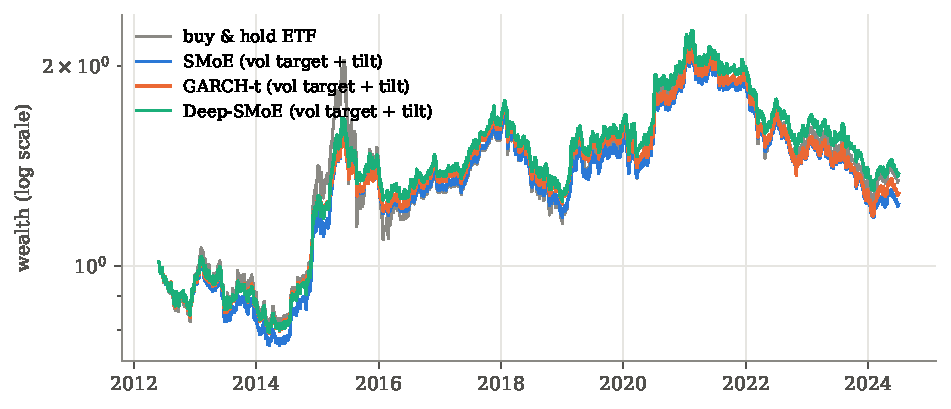
\includegraphics[width=\textwidth]{../results/figures/econ_equity_etf.pdf}
\caption{Wealth of the volatility-target-with-tilt rule on the CSI 300 ETF, net of costs, against
buy and hold.}\label{fig:equity}
\end{figure}

\begin{table}[!htbp]\centering\scriptsize
\caption{Trading results: CSI 300 ETF (510300), long-only, 3bp, out of sample}\label{tab:econ_etf510300}
\begin{adjustbox}{max width=\textwidth}
\begin{tabular}{llrrrrrrrrr}
\toprule
Model & Rule & Return & Vol & Sharpe & SE & MaxDD & Avg $w$ & Turnover & Excess CI lo & Excess CI hi\\
\midrule
Deep-SMoE & meanvar & 0.059 & 0.130 & 0.452 & 0.297 & -0.266 & 0.389 & 41.380 & -0.045 & 0.122\\
Gauss-HAR & meanvar & 0.034 & 0.111 & 0.304 & 0.294 & -0.230 & 0.375 & 14.048 & -0.082 & 0.106\\
SMoE & meanvar & 0.038 & 0.127 & 0.300 & 0.295 & -0.261 & 0.419 & 15.460 & -0.075 & 0.103\\
MAR & meanvar & 0.030 & 0.116 & 0.259 & 0.297 & -0.208 & 0.376 & 6.034 & -0.093 & 0.098\\
Chronos-Bolt-small & meanvar & 0.020 & 0.147 & 0.135 & 0.294 & -0.421 & 0.455 & 20.223 & -0.082 & 0.066\\
HistGauss & meanvar & 0.020 & 0.150 & 0.134 & 0.295 & -0.407 & 0.333 & 0.783 & -0.098 & 0.083\\
GARCH-t & meanvar & 0.016 & 0.156 & 0.102 & 0.293 & -0.476 & 0.806 & 0.845 & -0.065 & 0.052\\
Chronos-Bolt-small & sign & 0.046 & 0.171 & 0.271 & 0.295 & -0.397 & 0.541 & 38.255 & -0.049 & 0.090\\
Deep-SMoE & sign & 0.037 & 0.188 & 0.196 & 0.294 & -0.412 & 0.619 & 68.275 & -0.048 & 0.067\\
HistGauss & sign & 0.030 & 0.179 & 0.171 & 0.295 & -0.438 & 0.486 & 7.033 & -0.070 & 0.083\\
GARCH-t & sign & 0.025 & 0.226 & 0.112 & 0.293 & -0.463 & 1.000 & 0.000 & 0.000 & 0.000\\
MAR & sign & 0.003 & 0.178 & 0.018 & 0.293 & -0.447 & 0.595 & 20.585 & -0.092 & 0.047\\
Gauss-HAR & sign & -0.010 & 0.154 & -0.067 & 0.292 & -0.537 & 0.556 & 50.263 & -0.104 & 0.039\\
SMoE & sign & -0.014 & 0.178 & -0.081 & 0.292 & -0.459 & 0.581 & 29.334 & -0.108 & 0.020\\
HistGauss & voltarget & 0.026 & 0.164 & 0.158 & 0.293 & -0.419 & 0.786 & 0.490 & -0.040 & 0.043\\
GARCH-t & voltarget & 0.021 & 0.150 & 0.141 & 0.293 & -0.441 & 0.795 & 3.262 & -0.051 & 0.047\\
Chronos-Bolt-small & voltarget & 0.023 & 0.181 & 0.128 & 0.293 & -0.461 & 0.912 & 5.697 & -0.037 & 0.037\\
Deep-SMoE & voltarget & 0.018 & 0.151 & 0.118 & 0.293 & -0.434 & 0.803 & 8.872 & -0.057 & 0.042\\
SMoE & voltarget & 0.016 & 0.153 & 0.106 & 0.293 & -0.439 & 0.814 & 7.403 & -0.059 & 0.040\\
Gauss-HAR & voltarget & 0.015 & 0.153 & 0.101 & 0.293 & -0.434 & 0.813 & 9.140 & -0.061 & 0.041\\
MAR & voltarget & 0.015 & 0.152 & 0.098 & 0.293 & -0.433 & 0.810 & 10.543 & -0.062 & 0.041\\
Deep-SMoE & vt\_tilt & 0.027 & 0.158 & 0.173 & 0.293 & -0.425 & 0.813 & 9.437 & -0.038 & 0.046\\
HistGauss & vt\_tilt & 0.027 & 0.167 & 0.159 & 0.294 & -0.422 & 0.786 & 0.688 & -0.037 & 0.041\\
GARCH-t & vt\_tilt & 0.021 & 0.156 & 0.137 & 0.293 & -0.450 & 0.825 & 3.148 & -0.049 & 0.046\\
SMoE & vt\_tilt & 0.018 & 0.157 & 0.117 & 0.293 & -0.443 & 0.819 & 8.233 & -0.050 & 0.040\\
MAR & vt\_tilt & 0.018 & 0.156 & 0.115 & 0.293 & -0.437 & 0.817 & 11.022 & -0.051 & 0.040\\
Gauss-HAR & vt\_tilt & 0.018 & 0.153 & 0.115 & 0.293 & -0.435 & 0.812 & 9.188 & -0.056 & 0.041\\
Chronos-Bolt-small & vt\_tilt & 0.021 & 0.184 & 0.114 & 0.293 & -0.474 & 0.914 & 6.058 & -0.038 & 0.031\\
\bottomrule
\end{tabular}
\end{adjustbox}
\par\smallskip\begin{minipage}{\textwidth}\footnotesize
Buy and hold: Sharpe 0.112, maximum drawdown -0.463. Annualised; decisions at the close, execution at the next open. Excess CI: 95\% stationary-bootstrap interval of the annualised mean return in excess of buy and hold.
\end{minipage}
\end{table}
\begin{table}[!htbp]\centering\scriptsize
\caption{Trading results: IF futures, long/short, 2bp, out of sample}\label{tab:econ_if_main}
\begin{adjustbox}{max width=\textwidth}
\begin{tabular}{llrrrrrrrrr}
\toprule
Model & Rule & Return & Vol & Sharpe & SE & MaxDD & Avg $w$ & Turnover & Excess CI lo & Excess CI hi\\
\midrule
Deep-SMoE & meanvar & 0.067 & 0.156 & 0.430 & 0.376 & -0.261 & 0.094 & 97.980 & -0.089 & 0.203\\
Chronos-Bolt-small & meanvar & 0.045 & 0.170 & 0.267 & 0.372 & -0.269 & 0.092 & 44.951 & -0.099 & 0.200\\
MAR & meanvar & 0.036 & 0.140 & 0.255 & 0.375 & -0.206 & 0.117 & 13.509 & -0.112 & 0.188\\
Gauss-HAR & meanvar & 0.015 & 0.141 & 0.105 & 0.373 & -0.249 & 0.174 & 46.336 & -0.118 & 0.150\\
HistGauss & meanvar & 0.015 & 0.164 & 0.092 & 0.374 & -0.387 & 0.054 & 1.954 & -0.161 & 0.183\\
GARCH-t & meanvar & -0.006 & 0.163 & -0.036 & 0.373 & -0.472 & 0.853 & 1.168 & -0.043 & 0.014\\
SMoE & meanvar & -0.006 & 0.167 & -0.038 & 0.373 & -0.380 & 0.084 & 56.403 & -0.180 & 0.149\\
Chronos-Bolt-small & sign & 0.093 & 0.198 & 0.468 & 0.372 & -0.275 & 0.092 & 78.096 & -0.054 & 0.267\\
Deep-SMoE & sign & 0.084 & 0.199 & 0.420 & 0.374 & -0.273 & 0.243 & 138.900 & -0.060 & 0.223\\
HistGauss & sign & 0.021 & 0.199 & 0.107 & 0.374 & -0.450 & 0.044 & 10.041 & -0.166 & 0.208\\
MAR & sign & 0.019 & 0.196 & 0.098 & 0.374 & -0.430 & 0.199 & 38.490 & -0.146 & 0.177\\
GARCH-t & sign & 0.007 & 0.197 & 0.036 & 0.373 & -0.454 & 1.000 & 0.000 & 0.000 & 0.000\\
SMoE & sign & -0.048 & 0.199 & -0.240 & 0.372 & -0.489 & 0.163 & 64.151 & -0.226 & 0.120\\
Gauss-HAR & sign & -0.068 & 0.197 & -0.344 & 0.373 & -0.521 & 0.155 & 116.029 & -0.238 & 0.084\\
Deep-SMoE & voltarget & 0.002 & 0.157 & 0.015 & 0.373 & -0.428 & 0.853 & 8.430 & -0.031 & 0.021\\
Chronos-Bolt-small & voltarget & 0.003 & 0.184 & 0.014 & 0.373 & -0.460 & 0.952 & 4.643 & -0.017 & 0.008\\
MAR & voltarget & 0.000 & 0.159 & 0.003 & 0.373 & -0.427 & 0.865 & 10.071 & -0.033 & 0.020\\
Gauss-HAR & voltarget & -0.001 & 0.160 & -0.005 & 0.373 & -0.428 & 0.867 & 9.158 & -0.033 & 0.018\\
SMoE & voltarget & -0.001 & 0.161 & -0.009 & 0.373 & -0.432 & 0.870 & 7.578 & -0.034 & 0.016\\
GARCH-t & voltarget & -0.003 & 0.157 & -0.018 & 0.373 & -0.438 & 0.849 & 3.286 & -0.039 & 0.017\\
HistGauss & voltarget & -0.007 & 0.166 & -0.040 & 0.373 & -0.422 & 0.855 & 0.417 & -0.039 & 0.011\\
Deep-SMoE & vt\_tilt & 0.005 & 0.161 & 0.034 & 0.374 & -0.422 & 0.861 & 7.493 & -0.026 & 0.021\\
MAR & vt\_tilt & 0.001 & 0.161 & 0.003 & 0.373 & -0.429 & 0.869 & 10.172 & -0.033 & 0.020\\
Gauss-HAR & vt\_tilt & -0.000 & 0.160 & -0.003 & 0.373 & -0.428 & 0.867 & 9.130 & -0.034 & 0.018\\
Chronos-Bolt-small & vt\_tilt & -0.002 & 0.184 & -0.008 & 0.373 & -0.473 & 0.953 & 4.600 & -0.021 & 0.005\\
GARCH-t & vt\_tilt & -0.002 & 0.162 & -0.015 & 0.373 & -0.448 & 0.874 & 3.094 & -0.036 & 0.015\\
SMoE & vt\_tilt & -0.003 & 0.162 & -0.018 & 0.373 & -0.435 & 0.872 & 8.386 & -0.036 & 0.016\\
HistGauss & vt\_tilt & -0.007 & 0.165 & -0.045 & 0.373 & -0.425 & 0.853 & 0.624 & -0.041 & 0.010\\
\bottomrule
\end{tabular}
\end{adjustbox}
\par\smallskip\begin{minipage}{\textwidth}\footnotesize
Buy and hold: Sharpe 0.036, maximum drawdown -0.454. Annualised; decisions at the close, execution at the next open. Excess CI: 95\% stationary-bootstrap interval of the annualised mean return in excess of buy and hold.
\end{minipage}
\end{table}
\begin{table}[!htbp]\centering\small
\caption{Backtest overfitting diagnostics}\label{tab:overfit}
\begin{adjustbox}{max width=\textwidth}
\begin{tabular}{rp{3.5cm}rrp{3.5cm}rrr}
\toprule
Trials & Best (all costs) & Sharpe (all) & DSR (all) & Best at 3bp & Sharpe (3bp) & DSR (3bp) & PBO (3bp)\\
\midrule
1,440 & Deep-SMoE, meanvar, c0.0, g10.0, v0.8 & 0.583 & 0.565 & Gauss-HAR, meanvar, c3.0, g10.0, v0.8 & 0.498 & 0.758 & 0.514\\
\bottomrule
\end{tabular}
\end{adjustbox}
\par\smallskip\begin{minipage}{\textwidth}\footnotesize
DSR: deflated Sharpe ratio, the probability that the true Sharpe ratio exceeds the expected maximum of the trials under the null; values below 0.95 are not significant. PBO: probability of backtest overfitting by combinatorially symmetric cross-validation with 16 blocks.
\end{minipage}
\end{table}
